\documentclass{article}

\usepackage{ctex}
\usepackage{fancyhdr}
\usepackage{extramarks}
\usepackage{amsmath}
\usepackage{amsthm}
\usepackage{amssymb} 
\usepackage{amsfonts}
\usepackage{tikz}
\usepackage{url}
\usepackage{float}
\usepackage{bm}


%\usetikzlibrary{automata,positioning}

%
% Basic Document Settings
%

\topmargin=-0.45in
\evensidemargin=0in
\oddsidemargin=0in
\textwidth=6.5in
\textheight=9.0in
\headsep=0.25in


\pagestyle{fancy}
\lhead{\hmwkAuthorName}
\chead{\hmwkClass\ (\hmwkClassInstructor): \hmwkTitle}
\rhead{\schoolID}
\lfoot{}
\cfoot{\thepage}

\renewcommand\headrulewidth{0.4pt}
\renewcommand\footrulewidth{0.4pt}

\setlength\parindent{0pt}

%
% Create Problem Sections
%

\newcommand{\enterProblemHeader}[1]{
    \nobreak\extramarks{}{Problem \arabic{#1} continued on next page\ldots}\nobreak{}
    \nobreak\extramarks{Problem \arabic{#1} (continued)}{Problem \arabic{#1} continued on next page\ldots}\nobreak{}
}

\newcommand{\exitProblemHeader}[1]{
    \nobreak\extramarks{Problem \arabic{#1} (continued)}{Problem \arabic{#1} continued on next page\ldots}\nobreak{}
    \stepcounter{#1}
    \nobreak\extramarks{Problem \arabic{#1}}{}\nobreak{}
}

\setcounter{secnumdepth}{0}
\newcounter{partCounter}
\newcounter{homeworkProblemCounter}
\setcounter{homeworkProblemCounter}{1}
\nobreak\extramarks{Problem \arabic{homeworkProblemCounter}}{}\nobreak{}

%
% Homework Problem Environment
%
% This environment takes an optional argument. When given, it will adjust the
% problem counter. This is useful for when the problems given for your
% assignment aren't sequential. See the last 3 problems of this template for an
% example.
%
\newenvironment{homeworkProblem}[1][-1]{
    \ifnum#1>0
        \setcounter{homeworkProblemCounter}{#1}
    \fi
    \section{Problem \arabic{homeworkProblemCounter}}
    \setcounter{partCounter}{1}
    \enterProblemHeader{homeworkProblemCounter}
}{
    \exitProblemHeader{homeworkProblemCounter}
}

%
% Homework Details
%   - Title
%   - Due date
%   - Class
%   - Section/Time
%   - Instructor
%   - Author
%

\newcommand{\hmwkTitle}{Homework\ \#7}
\newcommand{\hmwkClass}{Pattern Recognition}
\newcommand{\hmwkClassInstructor}{Professor Wang Guijin}
\newcommand{\hmwkAuthorName}{{Qingyun~Fang} }
\newcommand{\schoolID}{{2017311003}}

\newcommand{\hs}{\hspace{2em}}
\newcommand{\vs}{\vspace{2ex}}
%
% Title Page
%

\title{
    \vspace{2in}
    \textmd{\textbf{\hmwkClass:\ \hmwkTitle}}\\
    %\normalsize\vspace{0.1in}\small{Due\ on\ \hmwkDueDate\ at 3:10pm}\\
    \vspace{0.5cm}\LARGE{\textit{\hmwkClassInstructor}}
    \vspace{4in}
}

\author{\hmwkAuthorName\\
{\schoolID}\\
Use \LaTeX ~in 5.6~2018} 


\date{}

\renewcommand{\part}[1]{\textbf{ Part \Alph{partCounter}}\stepcounter{partCounter}}

%
% Various Helper Commands
%


% Alias for the Solution section header
\newcommand{\solution}{\textbf{\Large Solution}}

% Probability commands: Expectation, Variance, Covariance, Bias
\newcommand{\E}{\mathrm{E}}
\newcommand{\Var}{\mathrm{Var}}
\newcommand{\Cov}{\mathrm{Cov}}
\newcommand{\Bias}{\mathrm{Bias}}

\linespread{1.5}

\begin{document}

\maketitle
\setcounter{page}{0}
\thispagestyle{empty}
\pagebreak

\section{Problem One}
{\kaishu{\large 正态分布时分类}}


\hs 设有符合正态分布的两类训练样本,并且设$P(\omega_1)=P(\omega_2)=0.5$,且$\omega_1$和$\omega_2$满足下列关系:
\begin{equation*}
\begin{split}
\omega_1&=\{(3,4)(3,8)(2,6)(4,6)\}\\
\omega_2&=\{(3,0)(3,-4)(1,-2)(5,-2)\}	
\end{split}
\end{equation*}
求识别函数、识别界面方程、作图。

\subsection{Solution}
{\kaishu{\large 识别函数}}
\hs 在多元正态函数概率型$(p({\bm x}|\omega_i)\sim N({\bm \mu}_i,\bm{\Sigma}_i),i=1,...,c)$,其判别函数为:
\begin{equation*}
g_i({\bm x}) = -\frac{1}{2}({\bm x}-{\bm \mu}_i)^{\rm T}{\bm{\Sigma}_i}^{-1}({\bm x}-{\bm \mu}_i)-\frac{d}{2}\ln2\pi -\frac{1}{2}\ln(|\bm{\Sigma}_i|)+\ln P(\omega_i)
\end{equation*}

\hs 将题目中的数据代入可得:

\begin{table}[htbp]
	\centering
	\begin{tabular}{cccc}
		\hline 
		参数 &  数值 & 参数 & 数值 \\
		\hline 
		${\bm \mu}_1$ &  $(3,6)^{\rm T}$ & $|\bm{\Sigma}_1|$   & 1   \\
		${\bm \mu}_2$ &  $(3,-2)^{\rm T}$ & $|\bm{\Sigma}_2|$   & 4 \\
		${\bm{\Sigma}_1}$ & $\left[ \begin{array}{cc}
		0.5 & 0 \\
		0& 2
		\end{array}\right]$ & ${\bm{\Sigma}_1}^{-1}$ & $\left[ \begin{array}{cc}
		2 & 0 \\
		0& 0.5
		\end{array}\right]$ \\
		${\bm{\Sigma}_2}$ & $\left[ \begin{array}{cc}
		2 & 0 \\
		0& 2
		\end{array}\right]$ & ${\bm{\Sigma}_1}^{-1}$ & $\left[ \begin{array}{cc}
		0.5 & 0 \\
		0& 0.5
		\end{array}\right]$ \\
		\hline
	\end{tabular}
\caption{参数表}
\end{table}

\hs 因此 $g_1({\bm x})$和$g_2({\bm x})$如下:

\begin{equation*}
\begin{split}
g_1({\bm x})&= -(x_1-3)^2-0.25(x_2-6)^2-\ln2\pi+ \ln 0.5 \\
g_2({\bm x})&= -0.25(x_1-3)^2-0.25(x_2+2)^2-\ln2\pi- \frac{1}{2}\ln 4+ \ln 0.5
\end{split}
\end{equation*}

{\kaishu{\large 识别界面}}

\hs 显然识别界面方程为$g_1({\bm x})=g_2({\bm x})$,将其化简可得:
\begin{equation*}
 y = \frac{3}{16}(x-3)^2-\frac{\ln 4 }{8} + 2
\end{equation*}


{\kaishu{\large 界面显示}}

最终的识别结果如下:
\begin{figure}[htbp]
	\centering
	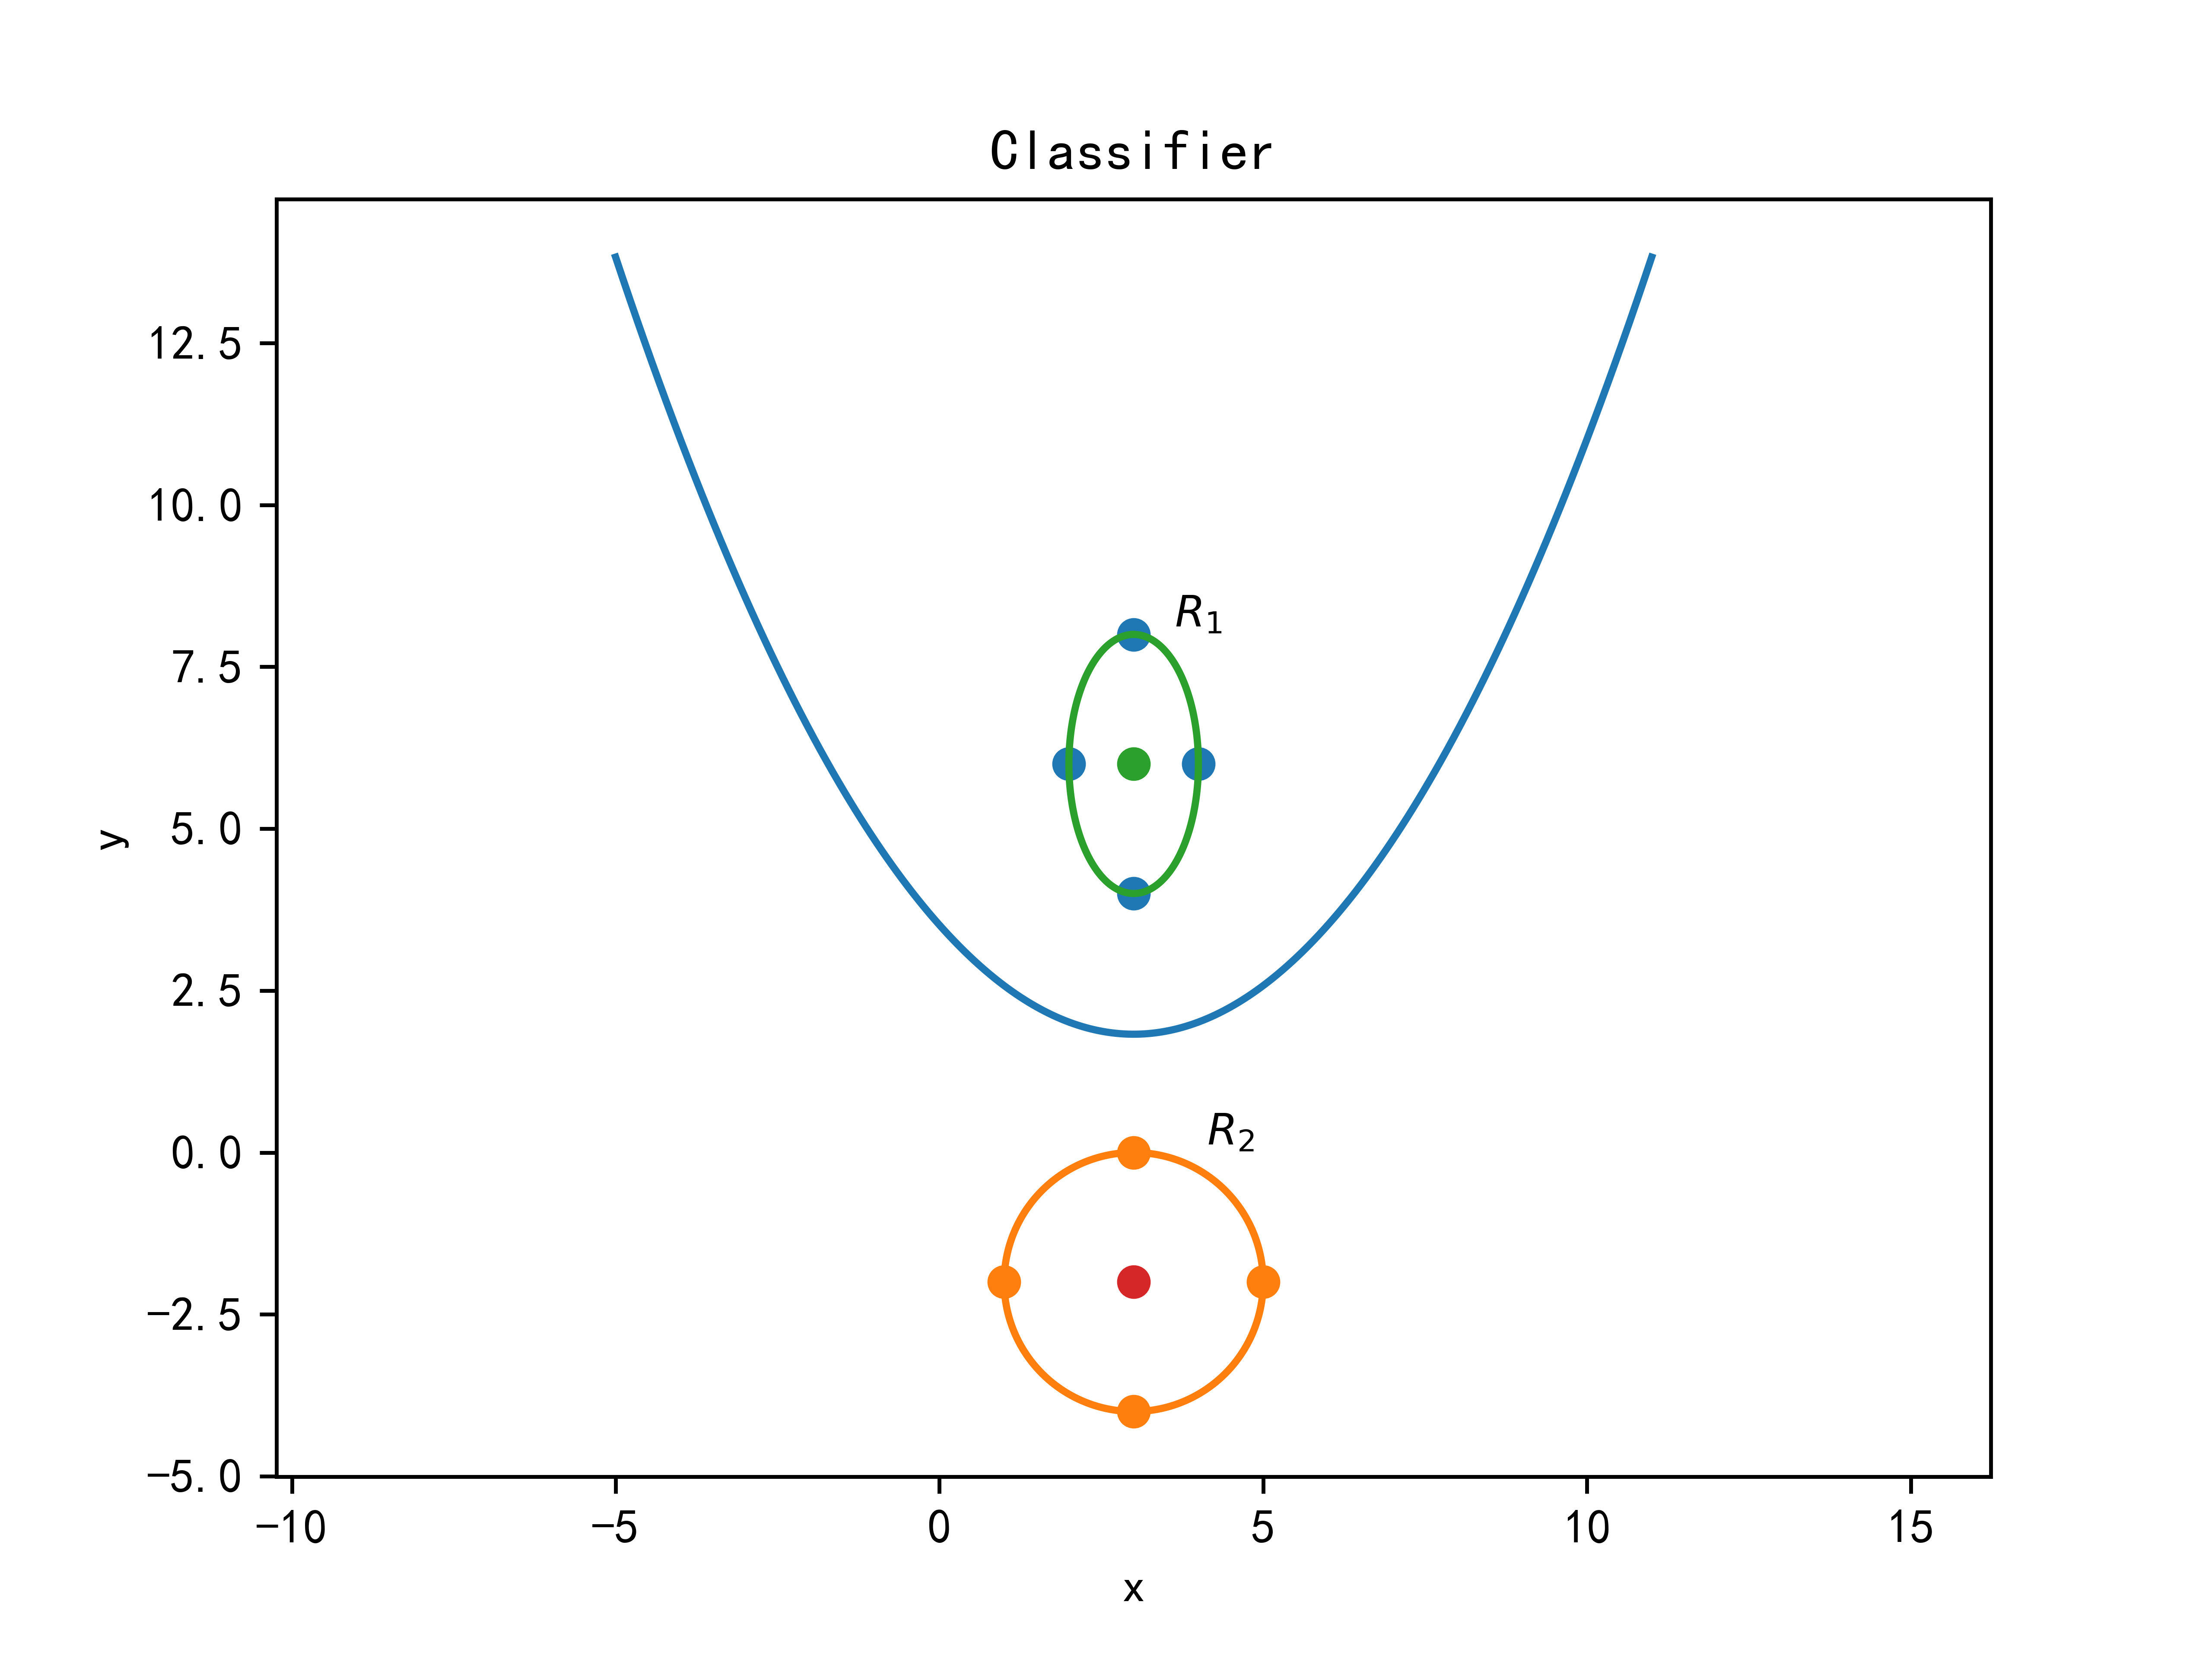
\includegraphics[width=0.6\linewidth]{img//fig1}
	\caption{识别结果}
\end{figure}

\hs 根据上图中$R_1$和$R_2$分别用来表征两类数据的等概率密度线,两类密度在$y$方向上具有相同的方差,仅在$x$上$P(\omega_1)$比$P(\omega_2)$小,因此$x$大的样本可能来自于$\omega_1$,并且其决策面为抛物线。\\

{\kaishu{\large 贝叶斯分类下错误率计算}}

\hs 在几类协方差不相同的情况下,其错误率很难用公式得出,因此在这里可以考虑用蒙特卡洛的方法来计算错误率。随机生成两维的正态分布数据,其方差和均值都满足表1。生成的数据分布如下图2:

\begin{figure}[H]
	\centering
	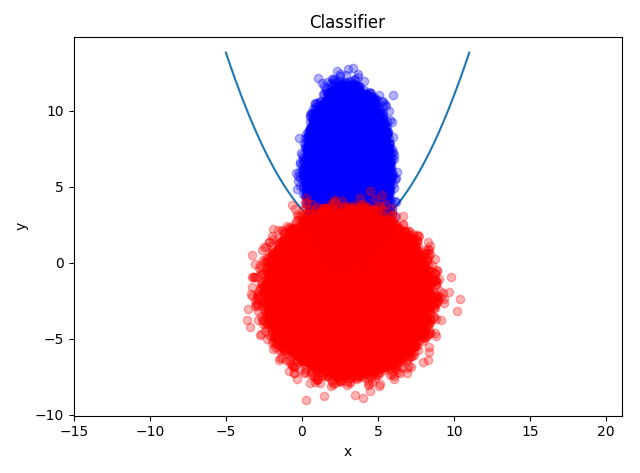
\includegraphics[width=0.6\linewidth]{img//fig2}
	\caption{随机数据分布}
\end{figure}

\hs 随机生成2000000个数据,每类都1000000个,统计错误率如下:
\begin{table}[htbp]
	\centering
	\begin{tabular}{cccc}
		\hline 
		类别 & 分类错误个数 &  精确率 & 召回率  \\
		\hline
		$\omega_1$ & 2001 & 99.7944\% & 99.7999\% \\
		$\omega_2$ & 2056 & 99.7999\% & 99.7944\% \\
		\hline
	\end{tabular}
	\caption{参数表}
\end{table}

\hs 运用蒙特卡洛法,得出的精确率和召回率都极其优秀,显示在数据分布为正态分布的前提下,运用贝叶斯决策的方法是十分有效的。\\

{\kaishu{\large 与Fisher准则对比}}

\hs Fisher准则虽然不对数据做任何假设,但是在很多情况下,投影到一维空间后其样本分布呈现一种正态分布的情况,显然二维空间中正态分布的数据在任意投影方向下都应该是正态分布的,因此Fisher准则处理这种数据应该有一种天然的优势。 

\hs  使用fisher准则分类,其投影方向为$y$轴,分界面为$y=2$,这一点从直观也可以判断出来,往$y$轴投影是类间距离最大的。 fisher 分类结果如下图3,其中黄色的直线为fisher分界面:
\begin{figure}[htbp]
	\centering
	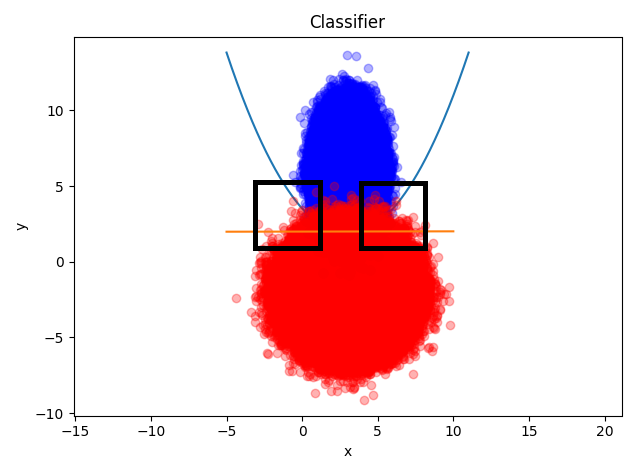
\includegraphics[width=0.6\linewidth]{img//fig3.png}
	\caption{Fisher 准则判断}
\end{figure}

\hs 接下来我们在统计一下Fisher的精准度和召回率,实验参数和之前的贝叶斯法相同:
\begin{table}[htbp]
	\centering
	\begin{tabular}{cccc}
		\hline 
		类别 & 分类错误个数 &  精确率 & 召回率  \\
		\hline
		$\omega_1$ & 2343 & 99.7773\% & 99.7657\% \\
		$\omega_2$ & 2262 & 99.7657\% & 99.7738\% \\
		\hline
	\end{tabular}
	\caption{参数表}
\end{table}

对比两种方法,贝叶斯的方法比Fisher准则的精度提升了一点,由于这些方法都是逼近与100\%的准确率,因此很难有大的提升了。在图3中用黑框标记出来了,这部分数据就是贝叶斯比Fisher准则优势的地方,性能的提升也就是靠这部分数据。
\end{document}
